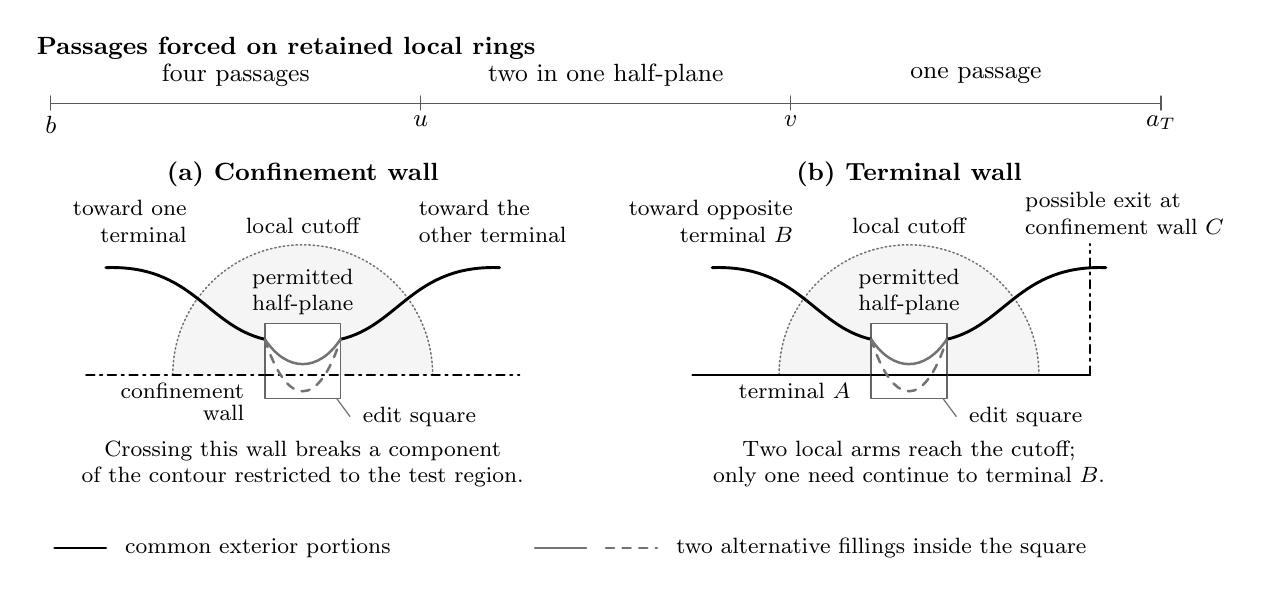
\begin{tikzpicture}[x=1cm,y=1cm,line cap=round,line join=round,
  every node/.style={font=\small},
  common/.style={black,line width=1.05pt},
  fillone/.style={black!55,line width=.9pt},
  filltwo/.style={black!55,line width=.9pt,dashed},
  cutoff/.style={black!55,line width=.55pt,densely dotted},
  confinement/.style={black,line width=.8pt,dash dot},
  terminal/.style={black,line width=.8pt}]

 \node[anchor=west,font=\small\bfseries] at (.15,6.6)
   {Passages forced on retained local rings};
 \draw[black!65] (.45,5.9)--(14.55,5.9);
 \foreach \x/\lab in {.45/b,5.15/u,9.85/v,14.55/a_T}{
   \draw[black!65] (\x,5.81)--(\x,5.99);
   \node[below,inner sep=2pt] at (\x,5.81) {$\lab$};
 }
 \node[align=center] at (2.8,6.25) {four passages};
 \node[align=center] at (7.5,6.25) {two in one half-plane};
 \node[align=center] at (12.2,6.25) {one passage};

 \begin{scope}[shift={(3.65,2.45)}]
  \node[font=\small\bfseries] at (0,2.55) {(a) Confinement wall};
  \fill[black!4] (-1.65,0) arc[start angle=180,end angle=0,radius=1.65]--cycle;
  \draw[cutoff] (-1.65,0) arc[start angle=180,end angle=0,radius=1.65];
  \node[font=\footnotesize] at (0,1.89) {local cutoff};
  \node[font=\footnotesize,align=center] at (0,1.05)
    {permitted\\half-plane};
  \draw[confinement] (-2.75,0)--(2.75,0);
  \node[anchor=east,font=\footnotesize] at (-.62,-.20) {confinement};
  \node[anchor=east,font=\footnotesize] at (-.62,-.48) {wall};
  \fill[white] (-.48,-.30) rectangle (.48,.65);
  \draw[black!60,line width=.55pt] (-.48,-.30) rectangle (.48,.65);
  \draw[confinement] (-.48,0)--(.48,0);
  \draw[common] (-2.5,1.36) .. controls (-1.4,1.4) and (-1.22,.62) .. (-.48,.45);
  \draw[common] (.48,.45) .. controls (1.22,.62) and (1.4,1.4) .. (2.5,1.36);
  \draw[fillone] (-.48,.45) .. controls (-.20,.03) and (.20,.03) .. (.48,.45);
  \draw[filltwo] (-.48,.45) .. controls (-.20,-.43) and (.20,-.43) .. (.48,.45);
  \node[font=\footnotesize,anchor=east,align=right] at (-1.35,1.95)
    {toward one\\terminal};
  \node[font=\footnotesize,anchor=west,align=left] at (1.35,1.95)
    {toward the\\other terminal};
  \draw[black!55,line width=.45pt] (.60,-.53)--(.43,-.30);
  \node[font=\footnotesize,anchor=west] at (.64,-.53) {edit square};
  \node[font=\footnotesize,align=center,text width=6.6cm] at (0,-1.13)
    {Crossing this wall breaks a component\\of the contour restricted to the test region.};
 \end{scope}

 \begin{scope}[shift={(11.35,2.45)}]
  \node[font=\small\bfseries] at (0,2.55) {(b) Terminal wall};
  \fill[black!4] (-1.65,0) arc[start angle=180,end angle=0,radius=1.65]--cycle;
  \draw[cutoff] (-1.65,0) arc[start angle=180,end angle=0,radius=1.65];
  \node[font=\footnotesize] at (0,1.89) {local cutoff};
  \node[font=\footnotesize,align=center] at (0,1.05)
    {permitted\\half-plane};
  \draw[terminal] (-2.75,0)--(2.30,0);
  \draw[confinement] (2.30,0)--(2.30,1.66);
  \node[anchor=east,font=\footnotesize] at (-.62,-.20) {terminal $A$};
  \fill[white] (-.48,-.30) rectangle (.48,.65);
  \draw[black!60,line width=.55pt] (-.48,-.30) rectangle (.48,.65);
  \draw[terminal] (-.48,0)--(.48,0);
  \draw[common] (-2.5,1.36) .. controls (-1.4,1.4) and (-1.22,.62) .. (-.48,.45);
  \draw[common] (.48,.45) .. controls (1.22,.62) and (1.4,1.4) .. (2.50,1.36);
  \draw[fillone] (-.48,.45) .. controls (-.20,.03) and (.20,.03) .. (.48,.45);
  \draw[filltwo] (-.48,.45) .. controls (-.20,-.43) and (.20,-.43) .. (.48,.45);
  \node[font=\footnotesize,anchor=east,align=right] at (-1.35,1.95)
    {toward opposite\\terminal $B$};
  \node[font=\footnotesize,anchor=west,align=left] at (1.35,2.05)
    {possible exit at\\confinement wall $C$};
  \draw[black!55,line width=.45pt] (.60,-.53)--(.43,-.30);
  \node[font=\footnotesize,anchor=west] at (.64,-.53) {edit square};
  \node[font=\footnotesize,align=center,text width=6.6cm] at (0,-1.13)
    {Two local arms reach the cutoff;\\only one need continue to terminal $B$.};
 \end{scope}

 \draw[common] (.5,.25)--(1.15,.25);
 \node[anchor=west,font=\footnotesize] at (1.27,.25) {common exterior portions};
 \draw[fillone] (6.6,.25)--(7.25,.25);
 \draw[filltwo] (7.5,.25)--(8.15,.25);
 \node[anchor=west,font=\footnotesize] at (8.27,.25) {two alternative fillings inside the square};
\end{tikzpicture}
